\chapter{TODO Non Fungible Tokens}
TODO

Even though the terms ``coins'' and ``tokens'' are often used interchangeably, they are not the same. Coins are fungible, meaning that they can be exchanged on a one-to-one basis. Tokens, on the other hand, \textit{may} be non-fungible, meaning that they are unique and cannot be exchanged on a one-to-one basis. This distinction is important because it has implications for how tokens are used and how they are valued.

Digital Tokens are non-native assets created on top of existing blockchains by smart contracts. Fungible tokens are interchangeable (20\$ bill may be exchanged for another 20\$ bill) and divisible (and mergeable), like cryptocurrencies.
A real-world example are casino tips, which are fungible, as they can be exchanged for other tips of the same value. 

\section{Non-fungible tokens}

Non-fungible tokens (NFTs) instead are unique and indivisible, like collectibles. NFTs are used to represent ownership of digital or physical assets, such as art, music, real estate, and more. They are created using smart contracts that define the rules for their creation, ownership, and transfer. NFTs are stored on the blockchain and can be bought, sold, and traded like any other asset. They are often used in online games, digital art, and other applications where ownership and scarcity are important.

\section{ERC standards}
The standard was needed to give developers the guarantee that assets will behave in a specific way and to ensure companies
that their tokens would be compatible with existing
Ethereum infrastructure such as wallets and exchanges.

ERC stands for Ethereum Request for Comments, and it is a set of standards that define how tokens should be created and managed on the Ethereum blockchain. The most popular ERC standards are ERC-20, ERC-721, and ERC-1155.
The latter allows for the creation of both fungible and non-fungible tokens, and is used in games and other applications where both types of tokens are needed. Tokens may also act ticket-like, meaning that they are fungible until some event date, and after it they become non fungible collectible tokens.

ICOs (Initial Coin Offerings) are a way to raise funds for a new project by selling tokens to investors. The tokens are usually created using the ERC-20 standard, which allows them to be traded on cryptocurrency exchanges. The ERC-20 standard defines how tokens should be created, transferred, and managed on the Ethereum blockchain. It also includes rules for how tokens should be stored and how they should be transferred between accounts.

DeFi (Decentralized Finance) tokens are used as ``collateral'' in lending and borrowing platforms, where users can borrow
funds by depositing their fungible tokens as ``collateral''.
They are used also for voting and governance in decentralized organizations, but also as a simple medium of exchange in financial transactions.\\ 
They represent  is a new way of doing finance that uses blockchain technology to create decentralized financial products and services. DeFi is built on the Ethereum blockchain and uses smart contracts to automate financial transactions. DeFi is often used to create lending and borrowing platforms, decentralized exchanges, and other financial products that are not controlled by a central authority.

\subsection{ERC-20}

\begin{paracol}{2}
   \colfill
   ERC-20 is the most widely used standard for creating tokens on the Ethereum blockchain. It defines a set of rules that tokens must follow in order to be compatible with the Ethereum ecosystem. These rules include how tokens should be created, transferred, and managed, as well as how they should be stored and how they should be transferred between accounts. ERC-20 tokens are \textbf{fungible}, meaning that they can be exchanged on a one-to-one basis. They are often used in ICOs and other applications where fungibility is important.
   \colfill
   \switchcolumn

   \begin{figure}[htbp]
      \centering
      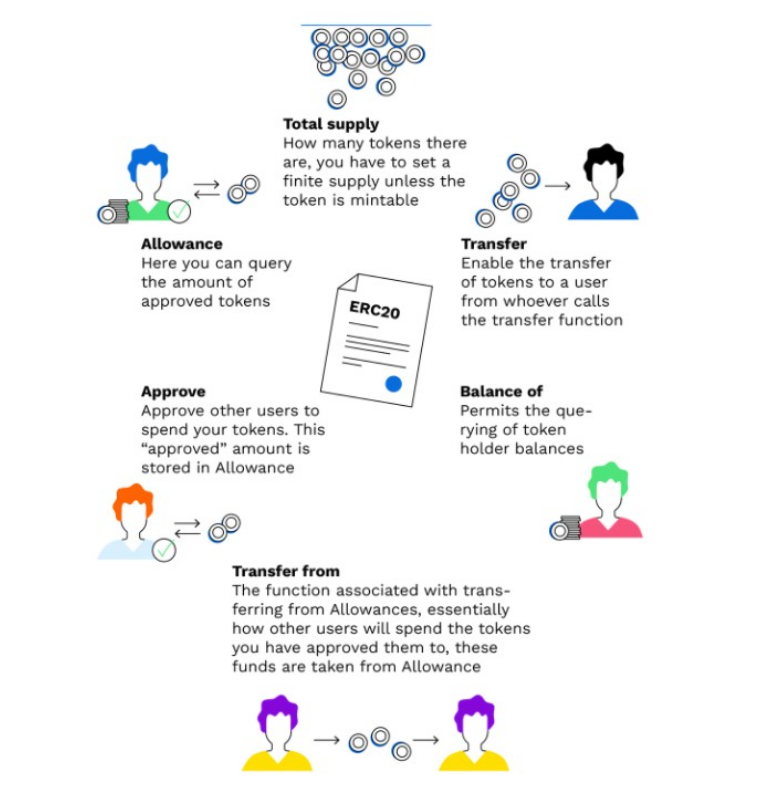
\includegraphics{images/erc20.png}
      \caption{ERC20 recap}
      \label{fig:erc20}
   \end{figure}

\end{paracol}
   
The token \textbf{contract} contains a map of account addresses and respective \textit{balances}.
The balance may differ from contract to contract, it may represent an amount of physical objects, rights, monetary value, etc.


ERC-20 tokens must implement the following functions:
\begin{itemize}
   \item \texttt{totalSupply()}: returns the total supply of tokens
   \item \texttt{balanceOf(address owner)}: returns the balance of tokens for a given address
   \item \texttt{transfer(address to, uint256 value)}: transfers tokens from the sender to the given address
   \item \texttt{transferFrom(address from, address to, uint256 value)}: transfers tokens from one address to another
   \item \texttt{approve(address spender, uint256 value)}: approves the given address to spend the sender's tokens
   \item \texttt{allowance(address owner, address spender)}: returns the amount of tokens that the spender is allowed to spend on behalf of the owner
\end{itemize}

Optional features include the \texttt{name()}, \texttt{symbol()}, and \texttt{decimals()} functions, which return the name, symbol, and number of decimal places for the token, respectively.
\nl

\textbf{Allowances} are used to allow one address to spend tokens on behalf of another address. This is useful for applications where tokens need to be transferred between accounts without the sender having to approve each transfer individually.
They are mostly used in decentralized exchanges (\texttt{DeFi} applications), where users can trade tokens without having to trust the exchange with their funds.
\framedt{Allowance example}{
   \begin{itemize}
      \item consider user A (Alice) and user B (Bob).
      \item A has 1000 tokens and want to give permission to B to spend 100 of them.
      \item A calls approve(address(B), 100)
      \item B checks how many tokens A gave him permission to use by calling allowance(address(A), address(B))
      \item  B sends to his account some of these tokens by calling transferFrom(address(A), address(B), 50)
      \item in subsequent withdrawals, B can finish withdrawing the rest of the funds, but he can only go up to 100 tokens, in total
   \end{itemize}
}

Minting and burning are the processes of creating and destroying tokens, respectively. These processes are often used in ICOs and other applications where tokens need to be created or destroyed on demand. The \texttt{mint()} and \texttt{burn()} Solidity (or OpenZeppelin) functions are used to create and destroy tokens, respectively.

\subsection{ERC-721}
ERC-721 is a standard proposed in 2018 for creating non-fungible tokens on the Ethereum blockchain. It defines a set of rules that tokens must follow in order to be compatible with the Ethereum ecosystem. These rules include how tokens should be created, transferred, and managed, as well as how they should be stored and how they should be transferred between accounts. ERC-721 tokens are \textbf{non-fungible}, meaning that they are unique and cannot be exchanged on a one-to-one basis. They are often used in online games, digital art, and other applications where ownership and scarcity are important.

All NFTs have a unique identifier \texttt{uint256} called \texttt{tokenId}, which is used to distinguish them from other tokens. This identifier is often a hash of the token's metadata, which includes information about the token's creator, owner, and other attributes. The metadata is stored off-chain and can be accessed by anyone who has the token's unique identifier.\\
For each NFT the pair \texttt{(address, uint256)} must be globally unique, with the \texttt{address} being the owner of the token.

\framedt{Transferring NFTs}{
   \begin{itemize}
      \item The owner ---Bob--- of an NFT can transfer it to another address by calling the \texttt{transferFrom(Bob,Alice, ID)} function on the token's contract.
      The ricipient address may be either an EOA or a contract, but in the latter case such contract must implement the \texttt{onERC721Received()} function, which provides an acknowledgement instrumental to the transaction's success.
      \item The owner of an NFT can also give permission to another address to transfer the token on their behalf by calling the \texttt{approve()} function on the token's contract.\\
      The approved address can then transfer the token to another address by calling the \texttt{transferFrom()} function.
   \end{itemize}
}
\nl

\textbf{Ongoing royalties }can be implemented by the contract, which will automatically send a percentage of the sale to the original creator of the NFT. This is done by implementing the \texttt{royaltyInfo()} function, which returns the percentage of the sale that should be sent to the creator.\\
On openSea the royalties are automatically managed by the platform on NFTs creation, and the creator can set the percentage of the sale that they want to receive as royalties.
\nl

The contract may include ---unlockable--- content that only the NFT owner can access, such as a link to a digital file or a message from the NFT creator. This is done by implementing the \texttt{tokenURI()} function, which returns the URI of the token's metadata. The metadata is stored off-chain and can be accessed by anyone who has the token's unique identifier.
\nl

\textbf{Contract metadata} is a JSON object that contains information about the token, such as its name, symbol, and other attributes. The metadata is stored off-chain and can be accessed by anyone who has the token's unique identifier. The metadata is often stored on IPFS or another decentralized storage platform to ensure that it is always available.
\note{Storing the data on-chain would be too expensive, as it would require a separate transaction for each token. It is used only if there is some information which must be persistently stored on-chain, such as the token's creator or owner.}